\documentclass{article}[a4paper,12pt]
\usepackage[utf8]{inputenc}
\usepackage{amsmath,amssymb,amsthm,amsfonts,mathtools}
\usepackage[inline]{enumitem}
\usepackage{soul}
\usepackage{cancel}
\usepackage{hyperref}
\usepackage{centernot}
\usepackage{pifont}
\usepackage{changepage}
\usepackage{subcaption}
\usepackage[section]{placeins}
\usepackage{lipsum, graphicx, caption}
\usepackage{float}
\usepackage{commath}
\usepackage{wrapfig}
\usepackage{amsmath}
\usepackage{amsfonts}
\usepackage{amssymb}
\theoremstyle{definition}
\newtheorem{innercustomgeneric}{\customgenericname}
\providecommand{\customgenericname}{}
\newcommand{\newcustomtheorem}[2]{%
  \newenvironment{#1}[1]
  {%
   \renewcommand\customgenericname{#2}%
   \renewcommand\theinnercustomgeneric{##1}%
   \innercustomgeneric
  }
  {\endinnercustomgeneric}
}
\newcustomtheorem{customthm}{Theorem}
\newcustomtheorem{customlem}{Lemma}
\newcustomtheorem{customdefn}{Definition}
\newcustomtheorem{customprop}{Proposition}
\newcustomtheorem{customexer}{Exercise}
\renewcommand{\qedsymbol}{$\blacksquare$}

\setlength\parindent{0pt}
\let\emptyset\varnothing
\usepackage{geometry}
\geometry{
	a4paper, portrait,
	total = {170mm,257mm},
	left = 20mm,
	top = 20mm,
}

\usepackage{xcolor}
\usepackage{pagecolor}
\pagecolor{white}
\color{black}

\title{\textbf{Neural Networks and Deep Learning}}
\author{
	\textbf{Om Prabhu}\\
	19D170018\\
	Undergraduate, Department of Energy Science and Engineering\\
	Indian Institute of Technology Bombay\\}
\date{Last updated \today}

\begin{document}
\maketitle
\vspace{-12pt}
\hrulefill
\vspace{6pt}

\textbf{NOTE:} This document is a brief compilation of my notes taken during the course `Neural Networks and Deep Learning'. You are free to use it and my project files for your own personal use \& modification. You may check out the course and/or specialization here: \texttt{\href{https://www.deeplearning.ai/}{deeplearning.ai}}.

\hrulefill
\tableofcontents
\vspace{6pt}

\hrulefill
\pagebreak

\section{Introduction}
\subsection{About myself}
Hello. I am Om Prabhu, currently an undergrad at the Department of Energy Science and Engineering, IIT Bombay. If you have gone through my website (\texttt{\href{https://omprabhu31.github.io/}{https://omprabhu31.github.io/}}) earlier, which is probably where you found this document too, you will know that I am quite a bit into programming and tinkering with code to try and do cool stuff. Additionally, I love playing video games, listening to music and engaging in a little bit of creative writing as and when I get time. With this brief self-introduction, let us get into why I decided to pursue this course.
\subsection{A little bit about deep learning}
As you probably know, deep learning has already transformed traditional internet businesses like web search and advertising. Further, it is also helping in the creation of businesses and business products and even jobs. Deep learning is making it into almost all types of industries ranging from healthcare and medical diagnosis to personalized education, precision agriculture and many others. 
\vspace{6pt}

Just as how electricity once transformed countless industries, AI today is on its way to doing the same. The part of AI that is contributing to most of this transformation is deep learning. This is a technical course which will teach us how to build neural networks and by the end of this course, we will be able to build a cat recognizer (for some reason, there is this cat meme running around in the world of AI which will also be discussed later).

\hrulefill
\pagebreak
\section{Overview of Deep Learning}
The terminology in AI is still not very well defined. For example, some people say that neural networks are a subset of deep learning while others use the two words almost interchangeably. Through most of this documentation, we will refer to deep learning as being a science of building and training neural networks. With that said, let's look at what a neural network is.
\subsection{Neural networks}
Let us use an example of demand prediction to try and understand what neural networks really are. Suppose a t-shirt company wants to know how many units they can expect to sell based on their selling price. The required dataset might be a in the form of a demand curve, where the higher the price the lesser the demand. This form of curve can be used to train what is perhaps the simplest possible neural network.
\begin{center}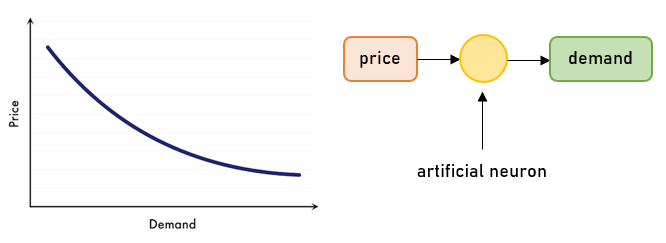
\includegraphics{deep_learning1.png}\end{center}
All this single-neuron network does is compute the curve shown and `learn' it in order to map any value of price to the appropriate value of demand. A single neuron can be thought of as a Lego brick, and a neural network as a very complicated stack, often in multiple layers, of such bricks.
\vspace{6pt}

Let's look at a more complicated example. Suppose that instead of just the price, we have more variables like shipping cost, marketing cost and material. Then we will have multiple factors that influence demand like affordability, consumer awareness and perceived quality. We might then have a slightly more complicated neural net like the one below:
\begin{center}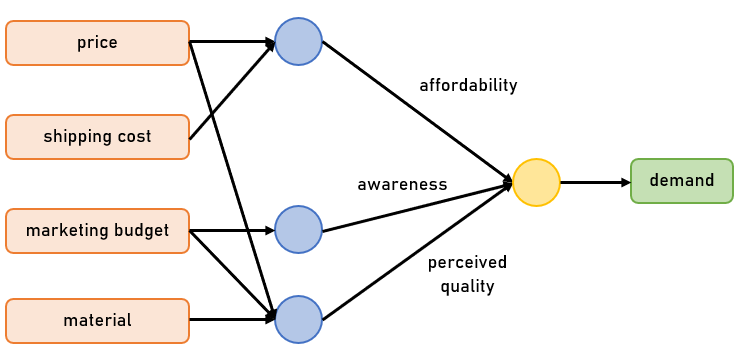
\includegraphics{deep_learning2.png}\end{center}
This slightly more complicated neural network maps the 4 input parameters to the output that is the demand.
\vspace{6pt}

From that the way in which we have discussed neural networks above, it appears as if we have to actually figure out the key factors as affordability, awareness and perceived quality. However, things do not work this way. One of the best things about neural networks is that we only have to provide it the input and the output $-$ all of the stuff in the middle, it figures out by itself. It automatically `learns' and completely trains itself to find the most accurate possible function that maps from the input to the output.
\vspace{6pt}

Another little correction is that it seems like the first node takes in only price and shipping inputs and so on. This is not the case. In practice, all nodes will be fed in with all the inputs and we let the individual neurons decide how many inputs they want to use and how they use them.
\subsection{Supervised learning with neural networks}
Most of the value created through deep learning has been in applications of supervised learning. This is the task of learning a function that maps an input to an output based on example input-output pairs (or A $\rightarrow$ B mapping). This has turned out to be very profitable for many industries such as:
\begin{itemize}
	\item online advertising: input is ad \& user info using which the algorithm tries to figure out if the user is likely to click on the ad
	\item computer vision: this is a very vast application area of AI (for example, input is an image and the algorithm tries to figure out whether the image is part of a dataset of 1000 images)
	\item speech recognition: input an audio clip and output a text transcript based on the input
	\item machine translation: input text or documents in certain languages and receive a translated output
	\item autonomous driving: AI algorithm uses image \& sensor info to figure out the position of nearby cars so it can avoid them
\end{itemize}
It turns out that slightly different types of neural networks are useful for different applications. For example, convolutional neural networks (CNN) are most commonly used for image applications while recurrent neural networks (RNN) are better for processing sequential data such as audio. More complicated applications often require the generation of custom neural network architecture.
\begin{center}
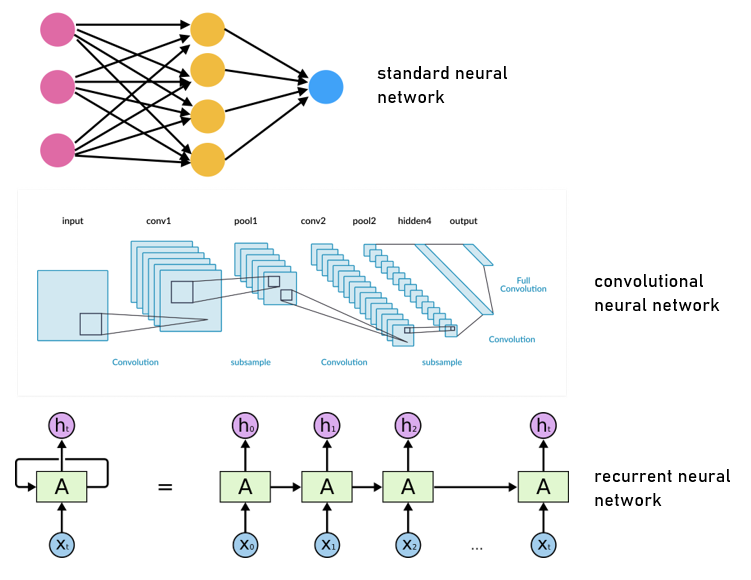
\includegraphics{types_of_nn.png}
\end{center}
Finally, supervised learning can be applied to both structured data (highly organized data such as tables, spreadsheets and databases) as well as unstructured data (data in the form of images, audio, video and even raw text).
\subsection{Why is deep learning taking off now?}
The ideas for deep learning and neural networks have been around for decades. Why is it that they have taken off only recently?
\vspace{6pt}

One of the major drivers of deep learning is scale. This refers to the ability of technology to train large sets of neural networks to process huge amounts of data while also improving AI performance. This can be illustrated through a graph as follows:
\begin{center}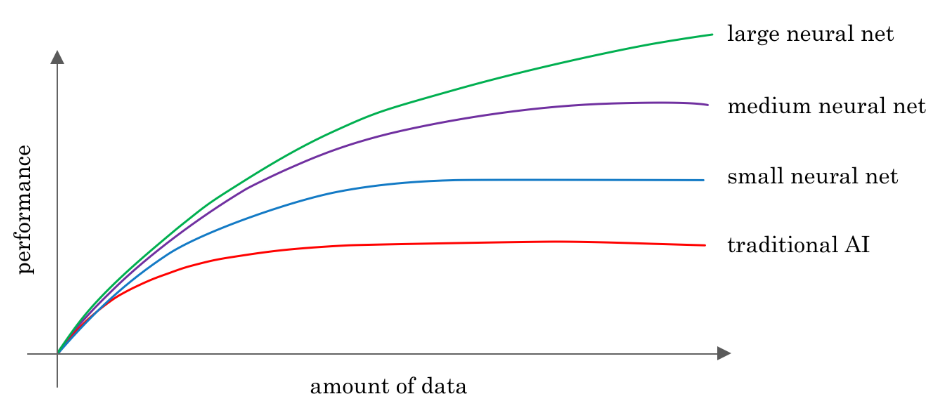
\includegraphics[scale=0.65]{data_vs_performance.png}\end{center}
\begin{itemize}
	\item for traditional deep learning systems, the data vs performance graph maxes out pretty early
	\item on training increasingly complex neural networks with higher amounts of data, performance keeps on getting better for much longer  
\end{itemize}
Hence to achieve the highest performance levels, we need two things. Firstly, it helps to have a lot of data. Additionally, we need the ability to train large sets of neural networks. Earlier, it was almost as if AI systems didn't know what to do with huge amounts of data. Now, with fast \& powerful CPUs and GPUs, it is possible for us to train large neural networks with a high amount of data.
\vspace{6pt}

Another factor is that of algorithmic innovation in order to increase the training speeds of neural networks. One of the major breakthroughs in this area has been the switch from sigmoid functions to ReLU functions:
\begin{center}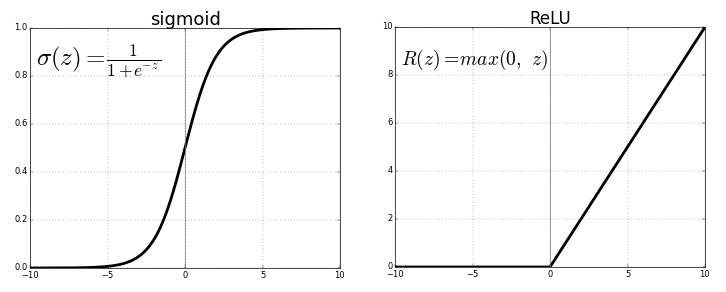
\includegraphics[scale=0.5]{sigmoid_relu.png}\end{center}
It turns out that on the tapering ends of the sigmoid function, since the gradient is nearly zero, the parameters hardly change and the training becomes very slow. In a ReLU curve, the gradient does not gradually shift to zero, so there is no point where the learning speed of the network is very slow. 
\vspace{6pt}

Fast computation is very important in deep learning, since the idea of training a neural network involves a lot of iterating $-$ basically we input the data, then train the neural network, then get feedback about how well the neural network performed, and then make changes to the data and neural network and repeat the cycle over and over until the neural network is trained well enough. Hence by reducing computation speeds, it leads to a huge rise in productivity while building out neural networks for AI projects.

\hrulefill
\begin{center}\textbf{END OF WEEK 1}\end{center}
This is the end of the course documentation from Week 1. Keep on reading further for documentation from further weeks, or spend some time gaining further insight into the previously discussed topics.

\hrulefill
\pagebreak
\section{Logistic Regression as a Neural Network}
\textit{(This section is currently in the works. Expect it to be up typically within a week's time.)}

\hrulefill

\end{document}
